\section{Wahrscheinlichkeitsmaße auf $\pmb{\R}$}
Kontinuierliche Ergebnisse lassen sich nicht mehr durch eine abzählbare Anzahl an Versuchsausgängen beschreiben.
Wahrscheinlichkeiten kann man dann nur noch \enquote{gutartigen Mengen} zuordnen, u.a.:
\begin{itemize}
	\item Intervalle sind gutartig
	\item Komplemente gutartiger Mengen sind gutartig
	\item Abzählbare Vereinigungen gutartiger Mengen sind gutartig
\end{itemize}
Bezeichne nun mit $\AG\subseteq\PG(\Omega)$ das System aller \enquote{gutartigen} Mengen.

\paragraph{Definition: $\boldsymbol{\sigma}$-Algebra}
Sei $\Omega\neq\emptyset$ ein beliebiger Grundraum. Eine Menge $\AG\subseteq\PG(\Omega)$ heißt $\boldsymbol{\sigma}$\textbf{-Algebra} auf $\Omega$, falls:
\begin{itemize}
	\item $\emptyset,\Omega\in\AG$
	\item $A\in\AG\implies A^{\mathsf{C}}\in\AG$
	\item $A_n\in\AG\;\forall n\in\N\implies\bigcup\limits_{n\in\N}A_n\in\AG$
\end{itemize}
$(\Omega,\AG)$ heißt dann \textbf{messbarer Raum}.
Die Mengen $A\in\AG$ heißen \textbf{Ereignisse}.

\paragraph{Definition: Borel-$\boldsymbol{\sigma}$-Algebra}
Die \textbf{Borel-$\boldsymbol{\sigma}$-Algebra} $\BG$ auf $\R$ beschreibt die kleinste $\sigma$-Algebra, welche alle Intervalle $(a,b]$ für beliebige $a,b\in\R$ enthält.

\paragraph{Definition: Wahrscheinlichkeitsmaß und Wahrscheinlichkeitsraum}
Sei $(\Omega,\AG)$ ein Messraum mit Grundraum $\Omega\neq\emptyset$ und $\sigma$-Algebra $\AG$.
Eine Abbildung $\PP:\AG\rightarrow[0,1]$ heißt Wahrscheinlichkeitsmaß auf $(\Omega,\AG)$, falls
\begin{itemize}
	\item $\PP(\Omega)=1$
	\item $A_n\in\AG,n\in\N$, disjunkt $\implies\PP(\bigcup\limits_{n\in\N}A_n)=\sum\limits_{n\in\N}\PP(A_n)$ \qquad($\sigma$-Additivität)
\end{itemize}
($\Omega,\AG,\PP$) heißt dann \textbf{Wahrscheinlichkeitsraum}.

\newpage
\paragraph{Sätze und Definitionen für allgemeine Wahrscheinlichkeitsräume}
Folgende Sätze und Definitionen übertragen sich sinngemäß, wobei als Ereignisse jeweils nur Mengen aus $\AG$ betrachtet werden:
\begin{itemize}
	\item \hyperref[rules]{Rechenregeln für diskrete Wahrscheinlichkeitsmaße}
	\item \hyperref[conditioned]{Bedingte Wahrscheinlichkeiten}
	\item \hyperref[bayes]{Satz von der Totalen Wahrscheinlichkeit und von Bayes}
	\item \hyperref[independant]{Stochastische Unabhängigkeit von Ereignissen}
\end{itemize}
\underline{Unterschied}: Während diskrete Wahrscheinlichkeitsmaße $\PP$ vollständig durch die Zähldichte $f(\omega)\coloneqq\PP(\{\omega\}),\omega\in\Omega$ bestimmt sind, ist dies für allgemeine Wahrscheinlichkeitsmaße falsch!

\paragraph{Definition: Verteilungsfunktion}
Ist $\PP$ ein Wahrscheinlichkeitsmaß auf $(\R,\BG_{\R})$, so gilt für die durch
\begin{tightcenter}
	$F:\R\rightarrow[0,1], F(x)\coloneqq\PP((-\infty,x])$
\end{tightcenter}
definierte \textbf{Verteilungsfunktion} von $\PP$:
\begin{itemize}
	\item $F$ ist monoton steigend
	\item $F$ ist rechtsseitig stetig
	\item $F(\infty)\coloneqq\lim\limits_{x\rightarrow\infty}F(x)=1, \; F(-\infty)\coloneqq\lim\limits_{x\rightarrow-\infty}F(x)=0$
\end{itemize}
Ist umgekehrt $F:\R\rightarrow[0,1]$ eine Funktion, die obige Punkte erfüllt, so existiert genau ein Wahrscheinlichkeitsmaß auf $(\R,\BG_{\R})$, das $F$ als Verteilungsfunktion besitzt.
Für ein diskretes Wahrscheinlichkeitsmaß $\PP$ ist die Verteilungsfunktion eine Treppenfunktion.

\paragraph{Definition: Dichten}
Sei $\PP$ ein Wahrscheinlichkeitsmaß auf $(\R,\BG_{\R})$. Existiert eine integrierbare Funktion $f:\R\rightarrow[0,\infty)$, sodass
\begin{tightcenter}
	$F(x)=\PP((-\infty,x])=\int_{-\infty}^{x}f(t)dt$ \qquad$\forall x\in\R$
\end{tightcenter}
so heißt $f$ Dichte von $\PP$ bzw. von der zugehörigen Verteilungsfunktion $F$.
Für $A\in\BG_{\R}$ gilt dann
\begin{tightcenter}
	$\PP(A)=\int_{\R}f(x)\cdot\mathds{1}_A(x)dx\eqqcolon\int_{A}f(x)dx$
\end{tightcenter}
Umgekehrt ist jede integrierbare Funktion $f:\R\rightarrow[0,\infty)$ mit $\int_{-\infty}^{\infty}f(t)dt=1$ Dichte eines Wahrscheinlichkeitsmaßes auf  $(\R,\BG_{\R})$, das durch obiges $F$ eindeutig festgelegt ist.
Falls eine Dichte existiert, ist $F$ stetig.

Achtung: Dichten dürfen nicht mit Zähldichten verwechselt werden!

\paragraph{Definition: Gleichverteilung}
Für $-\infty<a<b<\infty$ heißt das Wahrscheinlichkeitsmaß auf $(\R,\BG_{\R})$ zur Dichte $f\coloneqq\frac{1}{b-a}\mathds{1}_{(a,b]}$ \textbf{Gleichverteilung} $U_{(a,b]}$ auf $(a,b]$ und für $a\leq c<d\leq b$ gilt:\\ $U_{(a,b]}((c,d])=\frac{d-c}{b-a}$.

\paragraph{Definition: Exponentialverteilung}
Die \textbf{Exponentialverteilung} $Exp_\lambda$ mit Parameter $\lambda>0$ ist gegeben durch die Dichte
\begin{tightcenter}
	$f_\lambda(x)\coloneqq\frac{1}{\lambda}e^{-x/\lambda}\cdot\mathds{1}_{[0,\infty)}(x)$, \qquad$x\in\R$
\end{tightcenter}
Die Verteilungsfunktion ist gegeben durch $F_\lambda(x)=1-e^{-x/\lambda}$, \qquad$\forall x\geq 0$\\ und $F_\lambda(x)=0$ für alle $x<0$.

Exponentialverteilungen beschreiben Lebensdauern von Dingen, die nicht altern, d.h. die Wahrscheinlichkeit noch $y$ Jahre zu überleben, gegeben dass bereits $x$ Jahre überlebt wurden, hängt nicht von $x$ ab.

\paragraph{Definition: Normalverteilung}
Die \textbf{Normalverteilung} $N_{(\mu,\sigma^2)}$ mit Parametern $\mu\in\R,\sigma>0$ ist gegeben durch die Dichte
\begin{tightcenter}
	$f(x)\coloneqq\cfrac{1}{\sqrt{2\pi\sigma^2}}\cdot exp(-\cfrac{(x-\mu)^2}{2\sigma^2})$, \qquad$x\in\R$
\end{tightcenter}
Die Verteilung $N_{(0,1)}$ wird \textbf{Standardnormalverteilung} genannt.
Die Verteilungsfunktion von $N_{(0,1)}$ bezeichnet man mit
\begin{tightcenter}
	$\Phi(x)=\int_{-\infty}^{x}\frac{1}{\sqrt{2\pi}}e^{-t^2/2}dt$
\end{tightcenter}
Aufgrund der Symmetrie der Standardnormalverteilung zur y-Achse, gilt\\ $\Phi(-x)=1-\Phi(x)$ für alle $x\in\R$.
Insbesondere ist $\Phi(0)=\frac{1}{2}$.

Für die Verteilungsfunktion der Normalverteilung $N_{(\mu,\sigma^2)}$ gilt
\begin{tightcenter}
	$F(x)=\Phi(\frac{x-\mu}{\sigma})$
\end{tightcenter}
Um Wahrscheinlichkeiten für eine beliebige Normalverteilung zu berechnen, genügt also die Verteilungsfunktion $\Phi$ der Standardnormalverteilung:
\begin{center}
	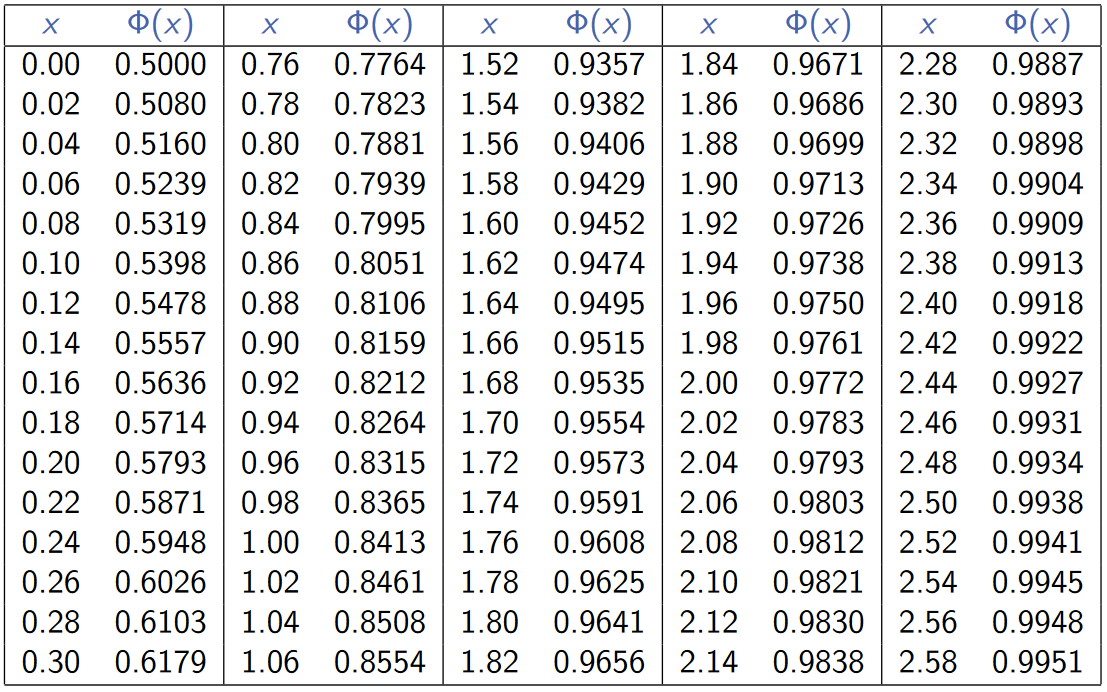
\includegraphics[width=0.8\textwidth]{images/image2.png}
\end{center}

\paragraph{Definition: Zufallsvariable, Messbarkeit und Verteilung}
Eine Zufallsvariable $X$ ist nur noch definiert, wenn das Urbild von $X$ eine \enquote{gutartige} Menge ist.

Seien $(\Omega,\AG)$, $(S,\CG)$ messbare Räume und $X:\Omega\rightarrow S$ eine Abbildung.
$X$ heißt $S$-wertige \textbf{Zufallsvariable}, falls $X^{-1}(C)\in\AG$ für alle $C\in\CG$ ist.\\
Man schreibt $X:(\Omega,\AG)\rightarrow(S,\CG)$ und sagt, dass $X$ $(\AG,\CG)$\textbf{-messbar} ist.
Die sogenannte \textbf{Verteilung} von $X$ unter $\PP$ wird durch das Wahrscheinlichkeitsmaß
\begin{tightcenter}
	$\PP^X(C)\coloneqq\PP(X^{-1}(C))=\PP(X\in C)$, \qquad$C\in\CG$
\end{tightcenter}
auf $(S,\CG)$ definiert.

\paragraph{Definition: Verteilungsfunktion und Dichte von Zufallsvariablen}
Sei $X:(\Omega,\AG)\rightarrow(S,\CG)$ eine $\R$-wertige Zufallsvariable auf dem Wahrscheinlichkeitsraum $(\Omega,\AG,\PP)$.
\begin{itemize}
	\item Die Verteilungsfunktion der Verteilung $\PP^X$ von $X$
	\begin{tightcenter}
		$F_X:\R\rightarrow[0,1],\; x\mapsto\PP^X((-\infty,x])=\PP(X\leq x)$
	\end{tightcenter}
	wird auch \textbf{Verteilungsfunktion} von $X$ genannt.
	\item $X$ heißt \textbf{stetige Zufallsvariable}, falls $F_X$ eine Dichte $f_X$ besitzt:
	\begin{tightcenter}
		$\PP(X\leq x)=\int_{-\infty}^{x}f_X(t)dt$ \qquad$\forall x\in\R$
	\end{tightcenter}
	$f_X$ heißt dann auch \textbf{Dichte} von $X$.
\end{itemize}

\paragraph{k$\boldsymbol{\sigma}$-Regeln für die Normalverteilung}
Für $X\sim N_{(\mu,\sigma^2)}$ und alle $t>0$ gilt
\begin{tightcenter}
	$\PP(|X-\mu|\leq\sigma t)=2\cdot\Phi(t)-1$
\end{tightcenter}
und insbesondere
\[   
\PP(|X-\mu|\leq k\sigma)=
\begin{cases}
	0,6827\;, & k=1\\
	0,9545\;, & k=2\\
	0,9973\;, & k=3
\end{cases}
\]

\paragraph{Definition: Borel-$\boldsymbol{\sigma}$-Algebren auf $\pmb{\R^n}$}
Borel-$\sigma$-Algebren, Verteilungsfunktion und Dichten kann man analog auch für $\Omega=\R^n$ definieren.
Die \textbf{Borel-$\boldsymbol{\sigma}$-Algebra} $\BG_{\R^n}$ auf $\R^n$ wird definiert als die kleinste $\sigma$-Algebra, die alle Rechteckmengen $\bigtimes\limits_{i=1}^{n}(a_i,b_i]$ mit $-\infty<a_i<b_i<\infty$ für alle $i\in\{1,\ldots,n\}$ enthält.

\paragraph{Definition: Multivariate Verteilungsfunktion}
Ist $\PP$ ein Wahrscheinlichkeitsmaß auf $(\R^n,\BG_{\R^n})$, so wird die zugehörige \textbf{multivariate Verteilungsfunktion} $F$ definiert durch
\begin{tightcenter}
	$F(x_1,\ldots,x_n)\coloneqq\PP(\bigtimes\limits_{i=1}^{n}(-\infty,x_i])$, \qquad$(x_1,\ldots,x_n)\in\R^n$
\end{tightcenter}

\paragraph{Definition: Dichten auf $\pmb{\R^n}$}
Sei $\PP$ ein Wahrscheinlichkeitsmaß auf $(\R^n,\BG_{\R^n})$ mit multivariater Verteilungsfunktion $F$.
Existiert eine Abbildung $f:\R^n\rightarrow[0,\infty)$, sodass für alle $(x_1,\ldots,x_n)\in\R^n$
\begin{tightcenter}
	$F(x_1,\ldots,x_n)=\int_{-\infty}^{x_1}\int_{-\infty}^{x_2}\cdots\int_{-\infty}^{x_n} f(t_1,\ldots,t_n)dt_n\ldots dt_2\,dt_1$
\end{tightcenter}
gilt, so heißt $f$ \textbf{Dichte} von $\PP$ bzw. von $F$.
\newpage
Es gilt dann $\forall B\in\BG_{\R^n}$
\begin{tightcenter}
	$\PP(B)=\int_{B}f(t)dt=\int_{-\infty}^{\infty}\cdots\int_{-\infty}^{\infty}\mathds{1}_B(t_1,\ldots,t_n)\cdot f(t_1,\ldots,t_n)dt_n\ldots dt_1$
\end{tightcenter}
Insbesondere gilt für jede Dichte $f$: $\int_{-\infty}^{\infty}\cdots\int_{-\infty}^{\infty}f(t_1,\ldots,t_n)dt_n\ldots dt_1=1$\\
und für $B=(a_1,b_1]\times\cdots\times(a_n,b_n],a_i<b_i$: $\PP(B)=\int_{a_1}^{b_1}\cdots\int_{a_n}^{b_n}f(t_1,\ldots,t_n)dt_n\ldots dt_1$.

\paragraph{Definition: Zufallsvektoren}
Ist $(\Omega,\AG)$ ein messbarer Raum und $X_i:\Omega\rightarrow\R,\,1\leq i\leq n$, so gilt $\forall1\leq i\leq n$:
\begin{tightcenter}
	$X=(X_1,\ldots,X_n):\Omega\rightarrow\R^n\;(\AG,\BG_{\R^n})$-messbar $\iff X_i:\Omega\rightarrow\R\;(\AG,\BG_{\R^n})$-messbar
\end{tightcenter}
In dem Fall wird $X$ auch $n$-dimensionaler \textbf{Zufallsvektor} genannt.
Die multivariate Verteilungsfunktion von $\PP^X$
\begin{tightcenter}
	$F_X(x_1,\ldots,x_n) \coloneqq\PP(X_1\leq x_1,X_2\leq x_2,\ldots,X_n\leq x_n)$
\end{tightcenter}
heißt \textbf{gemeinsame Verteilungsfunktion} von $X_1,\ldots,X_n$.
Besitzt $F_X$ eine Dichte $f_X$, dann heißt $X$ \textbf{stetig verteilt} und $f_X$ heißt \textbf{gemeinsame Dichte} von $X_1,\ldots,X_n$.
Es gilt dann $\PP^X(B)=\PP(X\in B)=\int_{B}f_X(t)dt$, \qquad$B\in\BG_{\R^n}$.

\paragraph{Definition: Randverteilungen}
Ist $X=(X_1,\ldots,X_n)$ ein Zufallsvektor auf $(\Omega,\AG,\PP)$, so heißen die Verteilungen $\PP^{X_i}$ \textbf{Randverteilungen/Marginalverteilungen}.
Die Verteilungsfunktion $F_i$ von $\PP^{X_i}$ bzw. $X_i$ berechnet sich wie folgt:
\begin{equation*}
	\begin{split}
		F_i(x) &= \PP(X_1<\infty,\ldots,X_{i-1}<\infty,X_i\leq x,X_{i+1}<\infty,\ldots,X_n<\infty) \\
		&= F(\infty,\ldots,\infty,x,\infty,\ldots,\infty),
	\end{split}
\end{equation*}	
wobei x an der $i$-ten Stelle steht.

\paragraph{Satz über die Dichte einer Komponente eines Zufallsvektors}
Besitzt die Zufallsvariable $X=(X_1,\ldots,X_n)$ eine gemeinsame Dichte $f:\R^n\rightarrow[0,\infty)$, so hat $X_i$ die Dichte $f_i:\R\rightarrow[0,\infty)$ mit
\begin{tightcenter}
	$f_i(x)=\int_{-\infty}^{\infty}\cdots\int_{-\infty}^{\infty}f(t_1,\ldots,t_{i-1},x,t_{i+1},\ldots,t_n)dt_n\cdots dt_{i+1}\,dt_{i-1}\cdots dt_1$
\end{tightcenter}
für alle $x\in\R$.

\paragraph{Definition: Unabhängigkeit von Zufallsvariablen}
Zufallsvariablen $X_1,\ldots,X_n:(\Omega,\AG)\rightarrow(\R,\BG_\R)$ heißen \textbf{stochastisch unabhängig}, wenn die Ereignisse $\{X_1\in B_1\},\ldots,\{X_n\in B_n\}$ für alle $B_1,\ldots,B_n\in\BG_\R$ stochastisch unabhängig sind.

\paragraph{Satz für stochastisch unabhängige Zufallsvariablen}
Für Zufallsvariablen $X_i:(\Omega,\AG)\rightarrow(\R,\BG_\R)$ mit Verteilungsfunktionen $F_{X_i}$ sind äquivalent:
\begin{itemize}
	\item $X_1,\ldots,X_n$ sind stochastisch unabhängig
	\item $\PP(X_1\in B_1,\ldots,X_n\in B_n)=\prod\limits_{i=1}^{n}\PP(X_i\in B_i)$ \qquad$\forall B_1,\ldots,B_n\in\BG_\R$
	\item  $\PP(X_1\leq x_1,\ldots,X_n\leq x_n)=\prod\limits_{i=1}^{n}\PP(X_i\leq x_i)=\prod\limits_{i=1}^{n}F_{X_i}(x_i)$ \qquad$\forall x_1,\ldots,x_n\in\R$
\end{itemize}
Zufallsvariablen sind also genau dann unabhängig, wenn die Verteilungsfunktion ihrer gemeinsamen Verteilung das Produkt ihrer Verteilungsfunktionen ist.

\paragraph{Dichten unabhängiger Zufallsvariablen}
Seien $X_i:\Omega\rightarrow\R$ für $i\in\{1,\ldots,n\}$ Zufallsvariablen auf einem Wahrscheinlichkeitsraum $(\Omega,\AG,\PP)$.
Falls alle Randverteilungen $\PP^{X_i}$ jeweils eine Dichte $f_i$ besitzen, dann sind äquivalent:
\begin{itemize}
	\item $X_1,\ldots,X_n$ sind stochastisch unabhängig:
	\item $\PP^{(X_1,\ldots,X_n)}$ besitzt eine Dichte $f$ gegeben durch $f(x_1,\ldots,x_n)\coloneqq\prod\limits_{i=1}^{n}f_i(x_i)$
\end{itemize}

\paragraph{Blockungslemma}
Seien $X_{11},X_{12},\ldots,X_{1n_1},X_{21},\ldots,X_{2n_2},\ldots,X_{k1},\ldots,X_{kn_k}$ stochastisch unabhängige Zufallsvariablen und $g_1:\R^{n_1}\rightarrow\R,g_2:\R^{n_2}\rightarrow\R,\ldots,g_k:\R^{n_k}\rightarrow\R$ Funktionen.
Dann sind auch die Zufallsvariablen
\begin{tightcenter}
	$Y_1\coloneqq g_1(X_{11}\ldots,X_{1n_1}),Y_2\coloneqq g_2(X_{21}\ldots,X_{2n_2}),\ldots,Y_k\coloneqq g_k(X_{k1}\ldots,X_{kn_k})$ 
\end{tightcenter}
stochastisch unabhängig.
Funktionen von disjunkten Blöcken unabhängiger Zufallsvariablen sind also wieder unabhängig.

\paragraph{Definition: Faltung für Verteilungen mit Dichten}
\begin{itemize}
	\item Sind $X,Y:(\Omega,\AG)\rightarrow(\R,\BG_\R)$ unabhängige Zufallsvariablen auf einem Wahrscheinlichkeitsraum $(\Omega,\AG,\PP)$ so wird die Verteilung $\PP^{X+Y}$ die \textbf{Faltung} von $\PP^X$ und $\PP^Y$ genannt.
	Schreibe dafür: $\PP^X*\PP^Y$
	\item Besitzt $X$ eine Dichte $f_X$ und $Y$ eine Dichte $f_Y$, so ist
	\begin{tightcenter}
		 $f_X*f_Y(z)=\int_{-\infty}^{\infty}f_X(x)f_Y(z-x)dx$, \qquad$z\in\R$
	\end{tightcenter}
	eine Dichte von $\PP^X*\PP^Y$, d.h. $f_{X+Y}=f_X*f_Y$
\end{itemize}

\paragraph{Definition: Gamma-Verteilung}
Die Zufallsvariable $X$ hat eine \textbf{Gamma-Verteilung} mit Parametern $\alpha>0$ und $\beta>0$, falls $X$ die Dichte
\begin{tightcenter}
	$f(t)=\frac{\beta^\alpha}{\Gamma(\alpha)}t^{\alpha-1}e^{-\beta t}\mathds{1}_{(0,\infty)}(t)$, \qquad$t\in\R$
\end{tightcenter}
mit Gamma-Funktion $\Gamma(t)\coloneqq\int_{0}^{\infty}x^{t-1}e^{-x}dx,\;t>0$ besitzt.

\paragraph{Additionsgesetze}
\begin{center}
	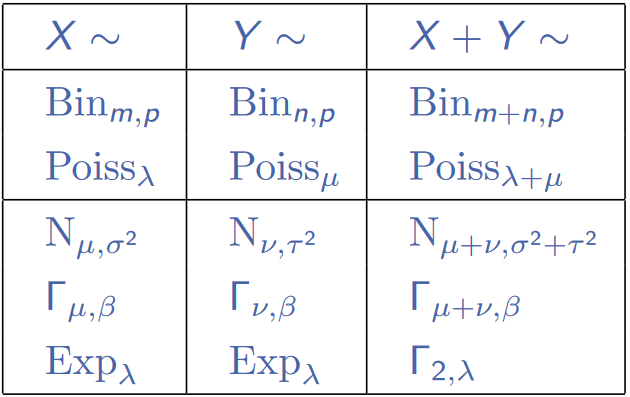
\includegraphics[width=0.3\textwidth]{images/image3.png}
\end{center}
\textbf{Beachte}: In jedem Fall sind $X$ und $Y$ als \underline{stochastisch unabhängig} vorausgesetzt.

\paragraph{Verteilungsfunktion von Maximum und Minimum}
Seien $X_1,\ldots,X_n$  stochastisch unabhängige Zufallsvariablen mit den Verteilungsfunktionen $F_{X_1},\ldots,F_{X_n}$.
Dann gilt:
\begin{itemize}
	\item $U\coloneqq max(X_1,\ldots,X_n)$ besitzt die Verteilungsfunktion 
	\begin{tightcenter}
		$F_U(t)=\prod\limits_{j=1}^{n}F_{X_j}(t)$, \qquad $t\in\R$
	\end{tightcenter}
	\item $V\coloneqq min(X_1,\ldots,X_n)$ besitzt die Verteilungsfunktion 
	\begin{tightcenter}
		$F_V(t)=1-\prod\limits_{j=1}^{n}(1-F_{X_j}(t))$, \qquad $t\in\R$
	\end{tightcenter}
\end{itemize}